\chapter{7}
\label{ch:7}

\todo[Name chapter, intro, discussion, summary]

INTRO

\section{Methodology}

For this study, we analyzed the relationship between user engagement and archival. In following the studies by Färber \cite{farber-jcdl2020} and Bhattarai et al. \cite{bhattarai-jcdl22} as well as our finding that 94\% of GHP URIs are to GitHub alone, we decided to focus on GitHub repository URIs. We used the GitHub API to extract engagement metrics for all GitHub repository URIs identified in Chapter 4. An example of the GitHub API response is shown in Appendix APDX. We used forks, subscribers, and stargazers metrics to define engagement. A fork is a new copy of the repository that is separately hosted in GitHub\footnote{\url{https://docs.github.com/en/pull-requests/collaborating-with-pull-requests/working-with-forks/about-forks}}. This is different from cloning the repository which makes a local copy of the repository on your local machine. Forks also allow for easy collaboration and interaction with the upstream repository that the repository was forked from. The terminology for watchers, subscribers, and stargazers has evolved. As of 2012, the watchers metric shown in the GitHub API has been split into two metrics: subscribers and stargazers\footnote{\url{https://docs.github.com/en/rest/activity/watching?apiVersion=2022-11-28}}. Subscribers have subscribed to notifications for activity in the repository while stargazers have bookmarked the repository but do not receive notifications. The subscriber terminology in the API response allows for continued support of watch endpoints in legacy apps\footnote{\url{https://github.blog/2012-09-10-watcher-api-changes/}}. In the browser UI, subscribers are shown as watchers (Figure \ref{fig:engagement_metrics}) which adds to the confusion with the terminology. For our purposes, we used the \verb|forks_count|, \verb|subscribers_count|, and \verb|stargazers_count| values from the GitHub API response.

\begin{figure}
    \centering
    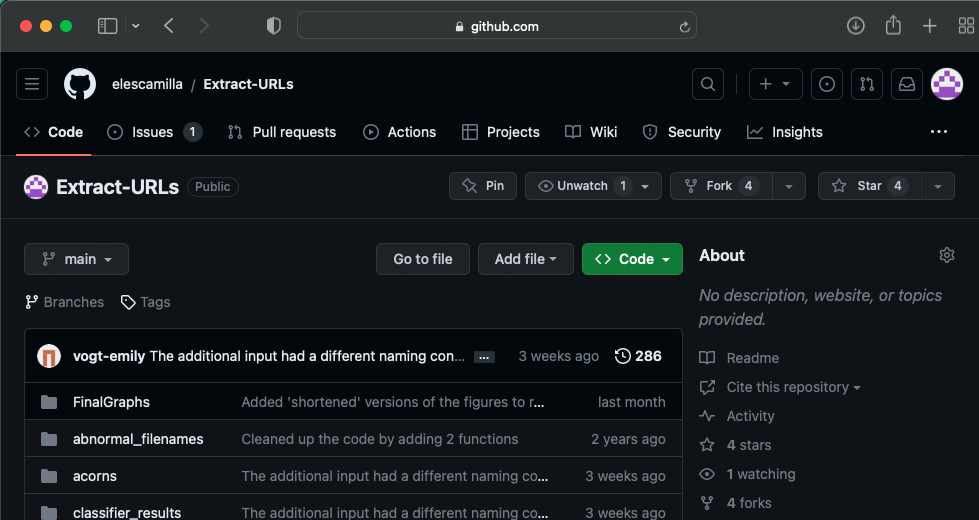
\includegraphics[width=\textwidth]{engagement_metrics.png}
    \caption{The engagement metrics are shown on the main page for each GitHub repository. Notice that the term ``watch'' is used in the browser UI.}
    \label{fig:engagement_metrics}
\end{figure}

We conducted the same statistical analysis as Bhattarai et al. \cite{bhattarai-jcdl22} by using a Mann Whitney U test to compare the distribution of the populations and Cliff's delta ($\delta$) to measure the effect size, or the strength of the relationship between two varWAbles in the population. The Mann-Whitney U test is a nonparametric test of the null hypothesis that, for randomly selected values X and Y from two populations, the probability of X being greater than Y is equal to the probability of Y being greater than X \cite{mannwhitney}. We established six null hypotheses, one for each engagement metric and archive:
\begin{enumerate}
\item For randomly selected fork counts X and Y from two populations (in SWH and not in SWH), the probability of X being greater than Y is equal to the probability of Y being greater than X. 
\item For randomly selected subscriber counts X and Y from two populations (in SWH and not in SWH), the probability of X being greater than Y is equal to the probability of Y being greater than X. 
\item For randomly selected stargazer counts X and Y from two populations (in SWH and not in SWH), the probability of X being greater than Y is equal to the probability of Y being greater than X. 
\item For randomly selected fork counts X and Y from two populations (in WA and not in WA), the probability of X being greater than Y is equal to the probability of Y being greater than X. 
\item For randomly selected subscriber counts X and Y from two populations (in WA and not in WA), the probability of X being greater than Y is equal to the probability of Y being greater than X. 
\item For randomly selected stargazer counts X and Y from two populations (in WA and not in WA), the probability of X being greater than Y is equal to the probability of Y being greater than X. 
\end{enumerate}
We used the Mann-Whitney U test function (\verb|mannwhitneyu()|) from SciPy\footnote{\url{https://docs.scipy.org/doc/scipy/reference/generated/scipy.stats.mannwhitneyu.html}} for each of three engagement metrics.

Cliff's Delta is a measure of how often the values in one distribution are larger than the values in a second distribution \cite{cliffsdelta}. If the Mann-Whitney U test answers the question``Is there a difference between the populations?'', Cliff's Delta answers the question ``How big is the difference?''. We used the \verb|cliffs-delta| Python package\footnote{\url{https://pypi.org/project/cliffs-delta/}} to implement the Cliff's delta calculation. We used the same categorization values used by Bhattarai et al. CITE to transform the numeric value to a meaningful category: negligible if $|\delta| < 0.12$, small if $|\delta| \in (0.12, 0.28)$, medium if $|\delta| \in (0.28, 0.43)$, and large if $|\delta| > 0.43$. The statistics for each population for each of the three engagement metrics is shown in Table \ref{tab:pop_stats}

\begin{table}[]
    \centering
    \begin{tabular}{|l|l|c|c|}
        \hline
        Metric & Archival Status & \multicolumn{1}{l|}{MedWAn} & \multicolumn{1}{l|}{Population Size} \\ \hline
        \multirow{4}{*}{Fork} & In SWH & 5 & 71,921 \\ \cline{2-4} 
         & Not In SWH & 2 & 37,054 \\ \cline{2-4} 
         & In WA & 4 & 105,816 \\ \cline{2-4} 
         & Not In WA & 1 & 26,723 \\ \hline
        \multirow{4}{*}{Subscribers} & In SWH & 4 & 71,921 \\ \cline{2-4} 
         & Not In SWH & 2 & 37,054 \\ \cline{2-4} 
         & In WA & 4 & 105,816 \\ \cline{2-4} 
         & Not In WA & 2 & 26,723 \\ \hline
        \multirow{4}{*}{Stargazers} & In SWH & 14 & 71,921 \\ \cline{2-4} 
         & Not In SWH & 6 & 37,054 \\ \cline{2-4} 
         & In WA & 14 & 105,816 \\ \cline{2-4} 
         & Not In WA & 4 & 26,723 \\ \hline
    \end{tabular}
\caption{Population statistics for each population for the three engagement metrics}
\label{tab:pop_stats}
\end{table}

\section{Results}

The numerical results of the Mann Whitney U test and Cliff's delta statistical analysis for each of the three engagement metrics and both archives is shown in Table \ref{tab:stat_analysis}. In this case, the p-value is so close to zero that it cannot be represented with a floating point. Therefore, there is nearly 100\% confidence that all six of the null hypotheses stated above can be rejected, indicating that there is a statistically significant difference between the distribution of each population. When comparing the populations of repositories archived in Software Heritage and not in Software Heritage, the effect size calculated with Cliff's delta and effect categorization show that both the number of forks and the number of stargazers are correlated with a medium difference between the two populations while the number of subscribers is correlated with a small difference between the two populations. The difference in the distributions is also shown in Figures \ref{fig:swh_forks}, \ref{fig:swh_subs}, and \ref{fig:swh_stars}. The repositories that have been archived in Software Heritage are indicated in orange while the repositories that have not been archived in Software Heritage are indicated in blue. The repositories that have been archived in Software Heritage have a longer tail than the repositories that have not been archived, showing that the repositories with higher engagement are more likely to be archived by Software Heritage. 

\begin{table}[]
    \centering
    \begin{tabular}{|l|l|c|c|c|c|}
        \hline
        Metric & Archive & \multicolumn{1}{l|}{U-value} & \multicolumn{1}{l|}{p-value} & \multicolumn{1}{l|}{Effect Size} & \multicolumn{1}{l|}{Effect Categorization} \\ \hline
        \multirow{2}{*}{Forks} & SWH & 143456778.5 & 0.0 & -0.31946 & Medium \\ \cline{2-6} 
         & WA & 1125018125.0 & 0.0 & -0.20429 & Small \\ \hline
        \multirow{2}{*}{Subscribers} & SWH & 157292028.0 & 0.0 & -0.25383 & Small \\ \cline{2-6} 
         & WA & 1113908954.5 & 0.0 & -0.21215 & Small \\ \hline
        \multirow{2}{*}{Stargazers} & SWH & 142883042.0 & 0.0 & -0.32218 & Medium \\ \cline{2-6} 
         & WA & 1125201331.5 & 0.0 & -0.20416 & Small \\ \hline
    \end{tabular}
\caption{Results of the statistical analysis for each of the three engagement metrics: forks, subscribers, and stargazers}
\label{tab:stat_analysis}
\end{table}

\begin{figure}
    \centering
    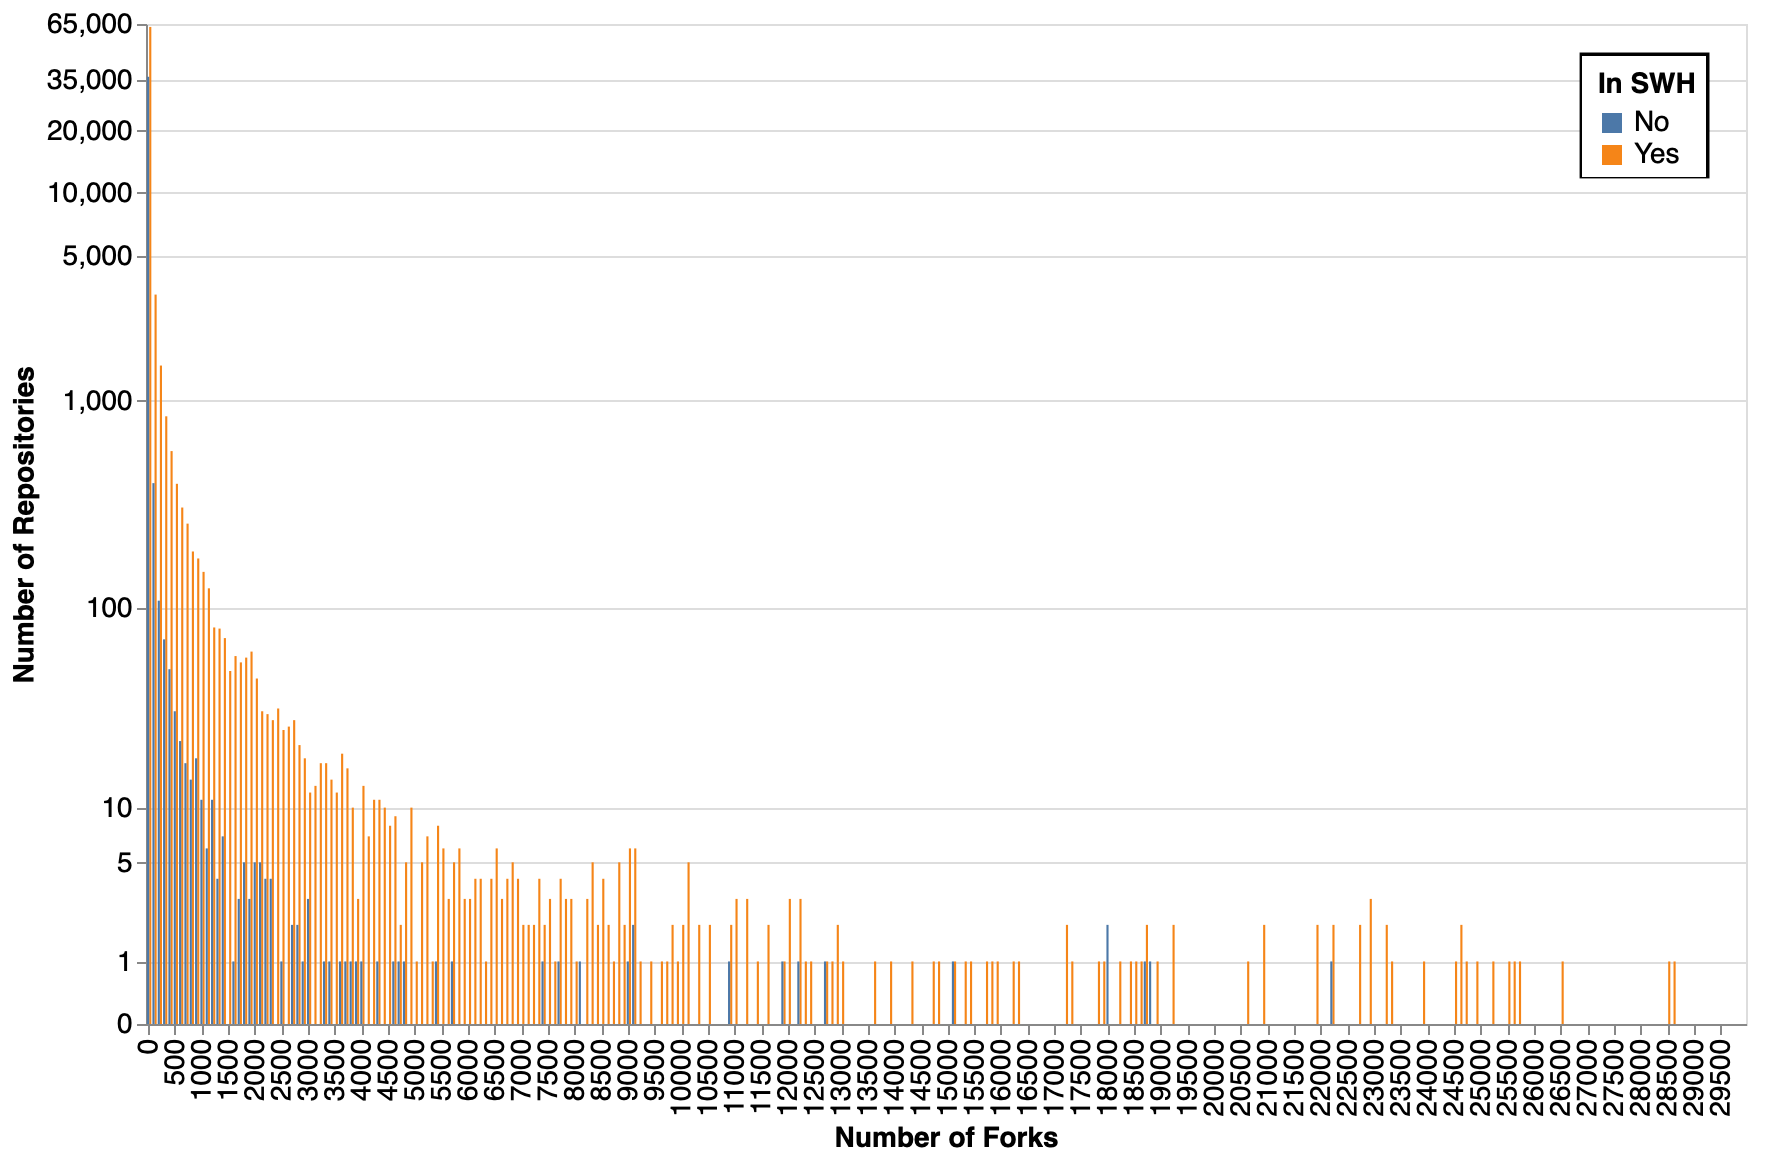
\includegraphics[width=\textwidth]{swh_forks.png}
    \caption{The distribution of forks for repositories archived and not archived in Software Heritage}
    \label{fig:swh_forks}
\end{figure}

\begin{figure}
    \centering
    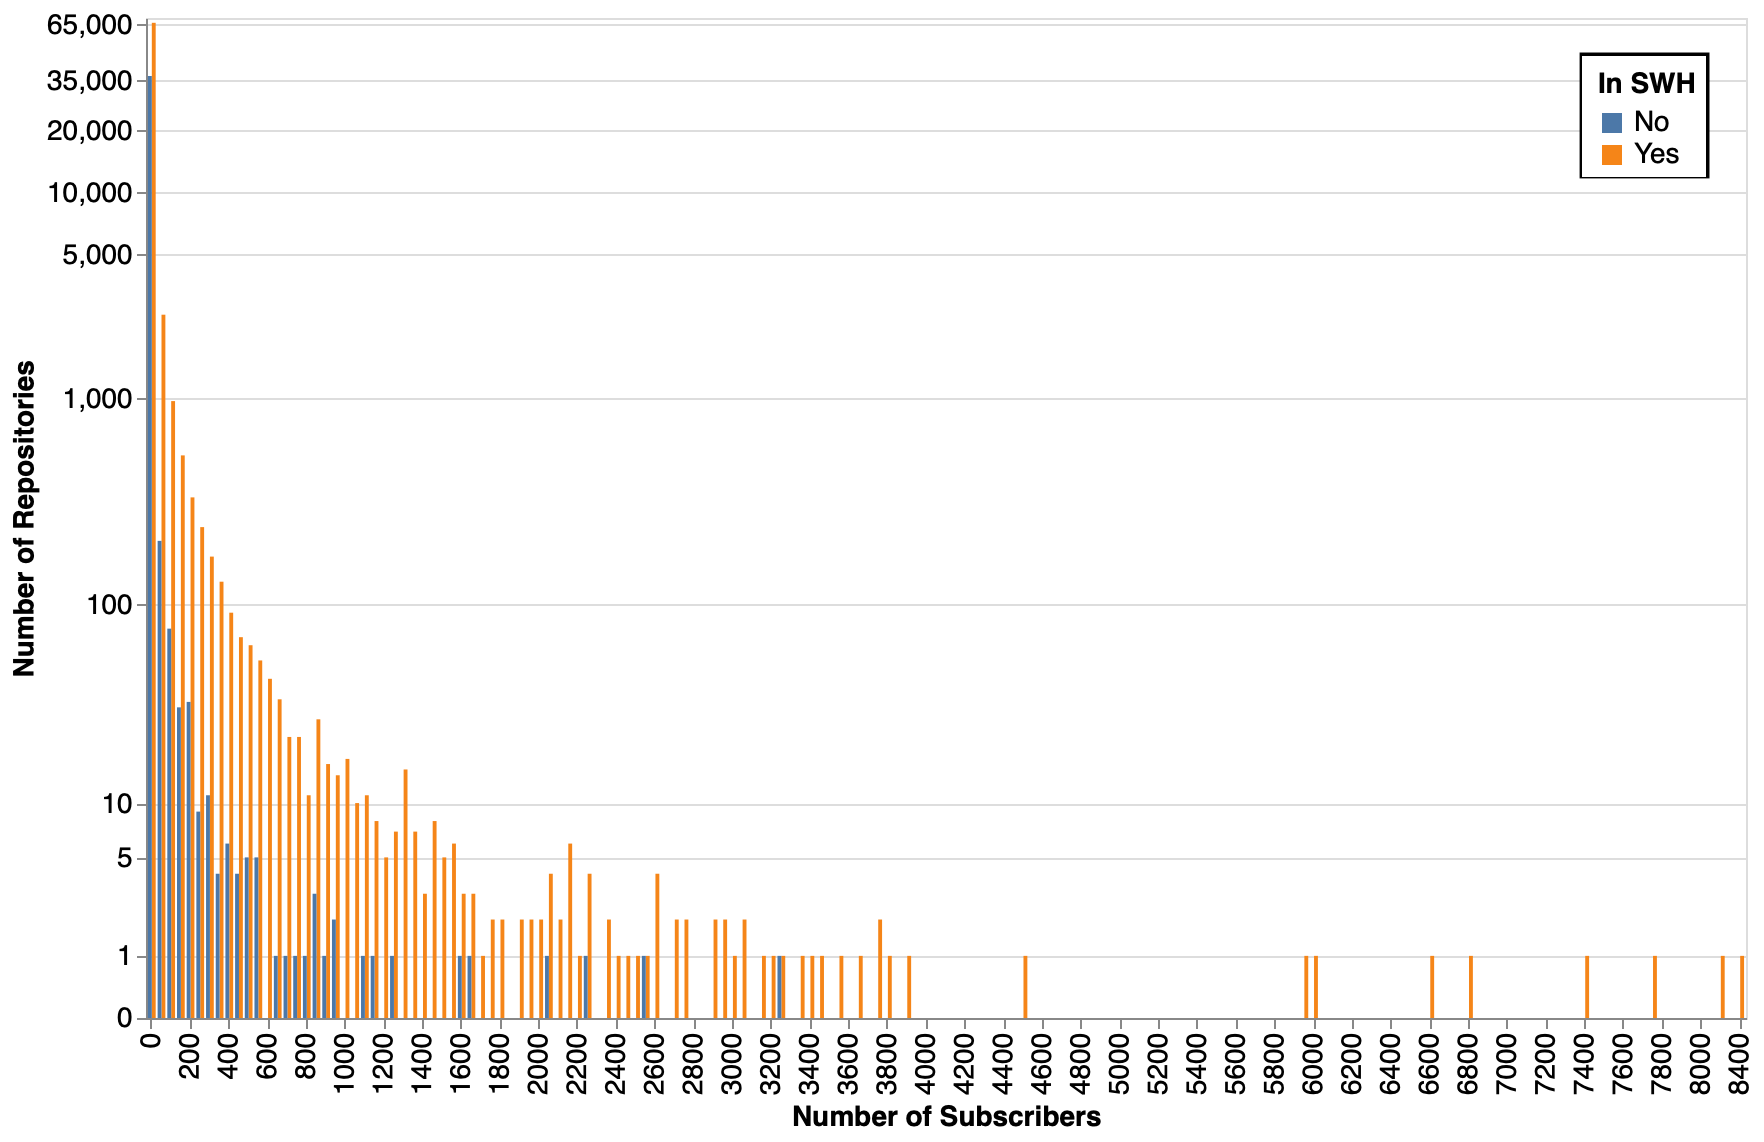
\includegraphics[width=\textwidth]{swh_subs.png}
    \caption{The distribution of subscribers for repositories archived and not archived in Software Heritage}
    \label{fig:swh_subs}
\end{figure}

\begin{figure}
    \centering
    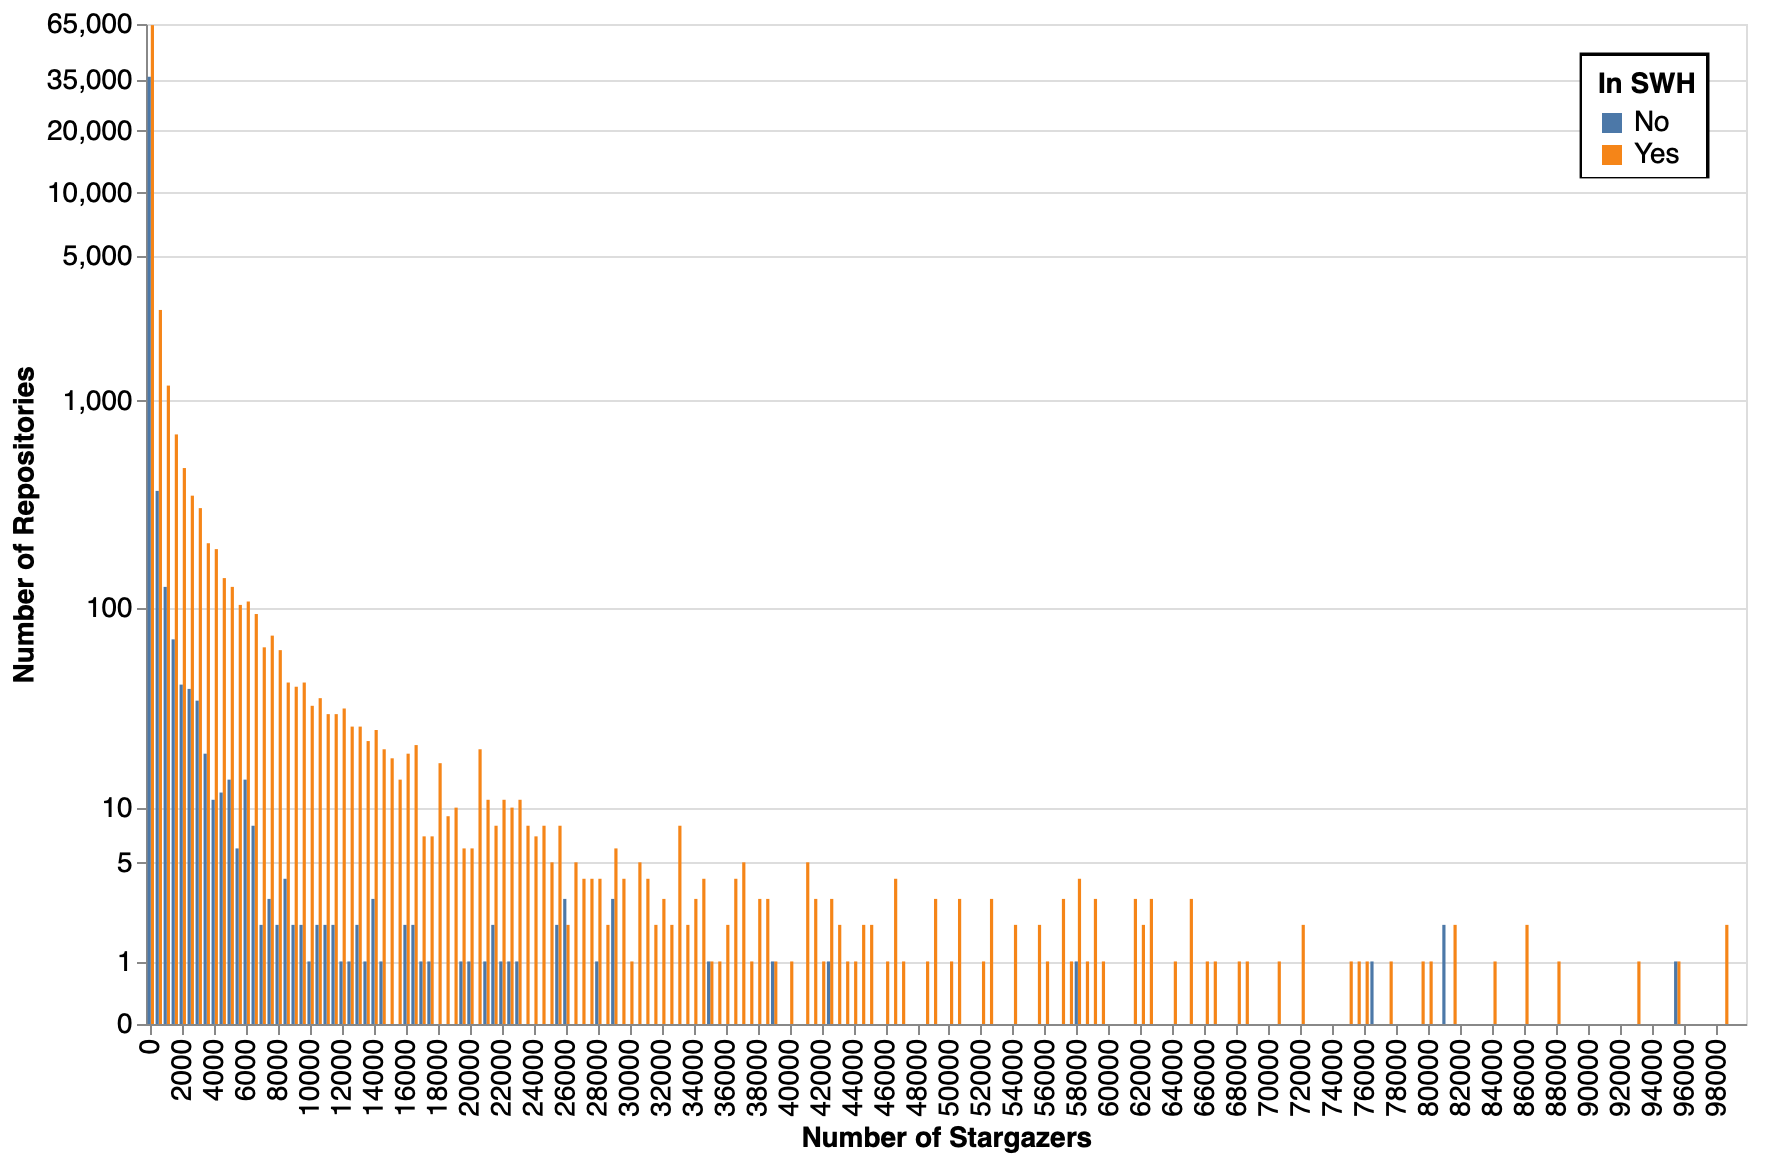
\includegraphics[width=\textwidth]{swh_stars.png}
    \caption{The distribution of stargazers for repositories archived and not archived in Software Heritage}
    \label{fig:swh_stars}
\end{figure}

As shown in Table \ref{tab:stat_analysis}, the effect size was categorized as small for all three engagement metrics when comparing repositories archived by Web archives and not archived by Web archives. Additionally, Cliff's delta can be understood as the probability that a randomly selected value from one group is larger than a randomly selected value from the second group. Therefore, for the subscribers engagement metric, there is a one in four change that the number of subscribers for a randomly selected repository that has not been archived by Software Heritage will be less than the number of subscribers for a randomly selected repository that has been archived by Software Heritage. This understanding adds context to the effect size for the Web archives populations. For all three metrics, the probability that a randomly selected repository that is not in the Web archives will have a smaller engagement value than a randomly selected repository that is in the Web archives is one in five. This decrease in the effect size can be seen when we use a histogram to plot the engagement metrics for each population as shown in Figures \ref{fig:wa_forks}, \ref{fig:wa_subs}, and \ref{fig:wa_stars}. The repositories that have been archived in Web archives are indicated in orange while the repositories that have not been archived in Web archives are indicated in blue. Unlike the Software Heritage populations, the distinctions between in the Web archives populations is not as clear for all three engagement metrics. 

\begin{figure}
    \centering
    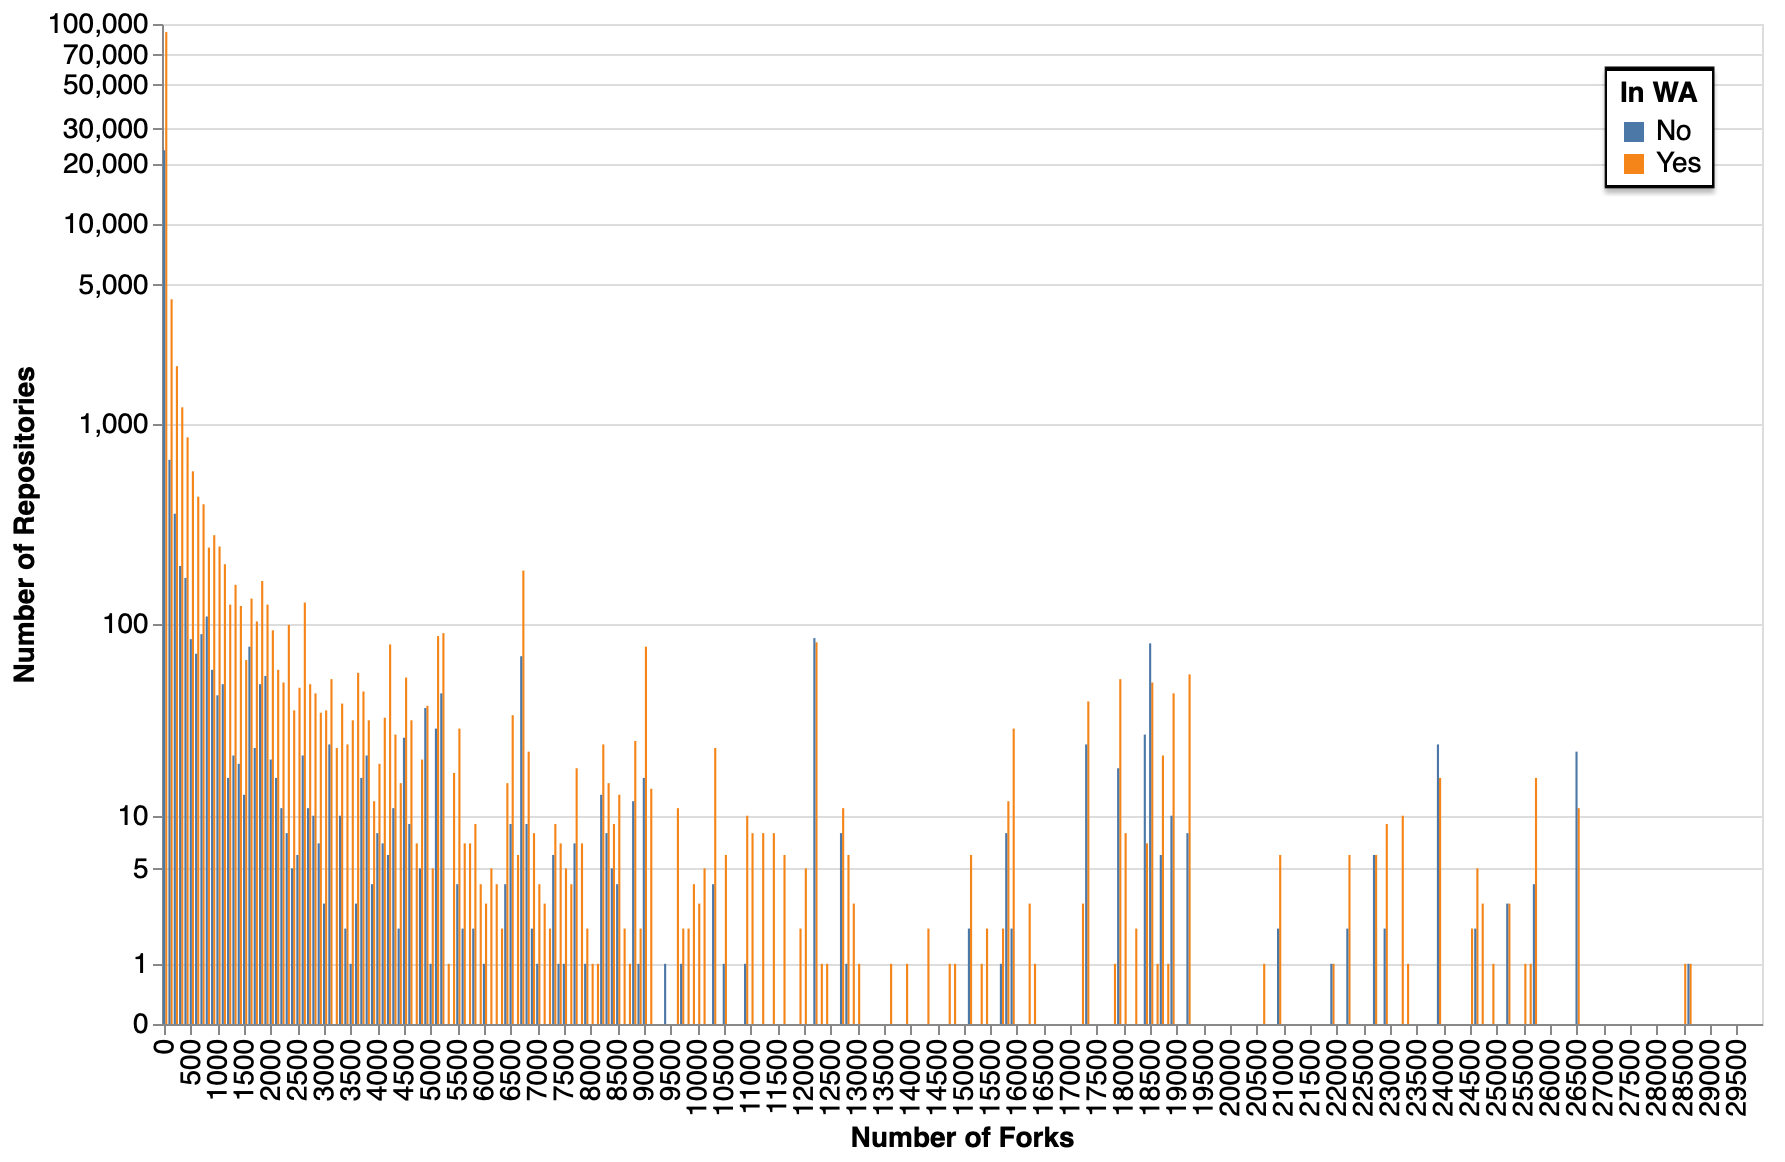
\includegraphics[width=\textwidth]{wa_forks.png}
    \caption{The distribution of forks for repositories archived and not archived in Web archives}
    \label{fig:wa_forks}
\end{figure}

\begin{figure}
    \centering
    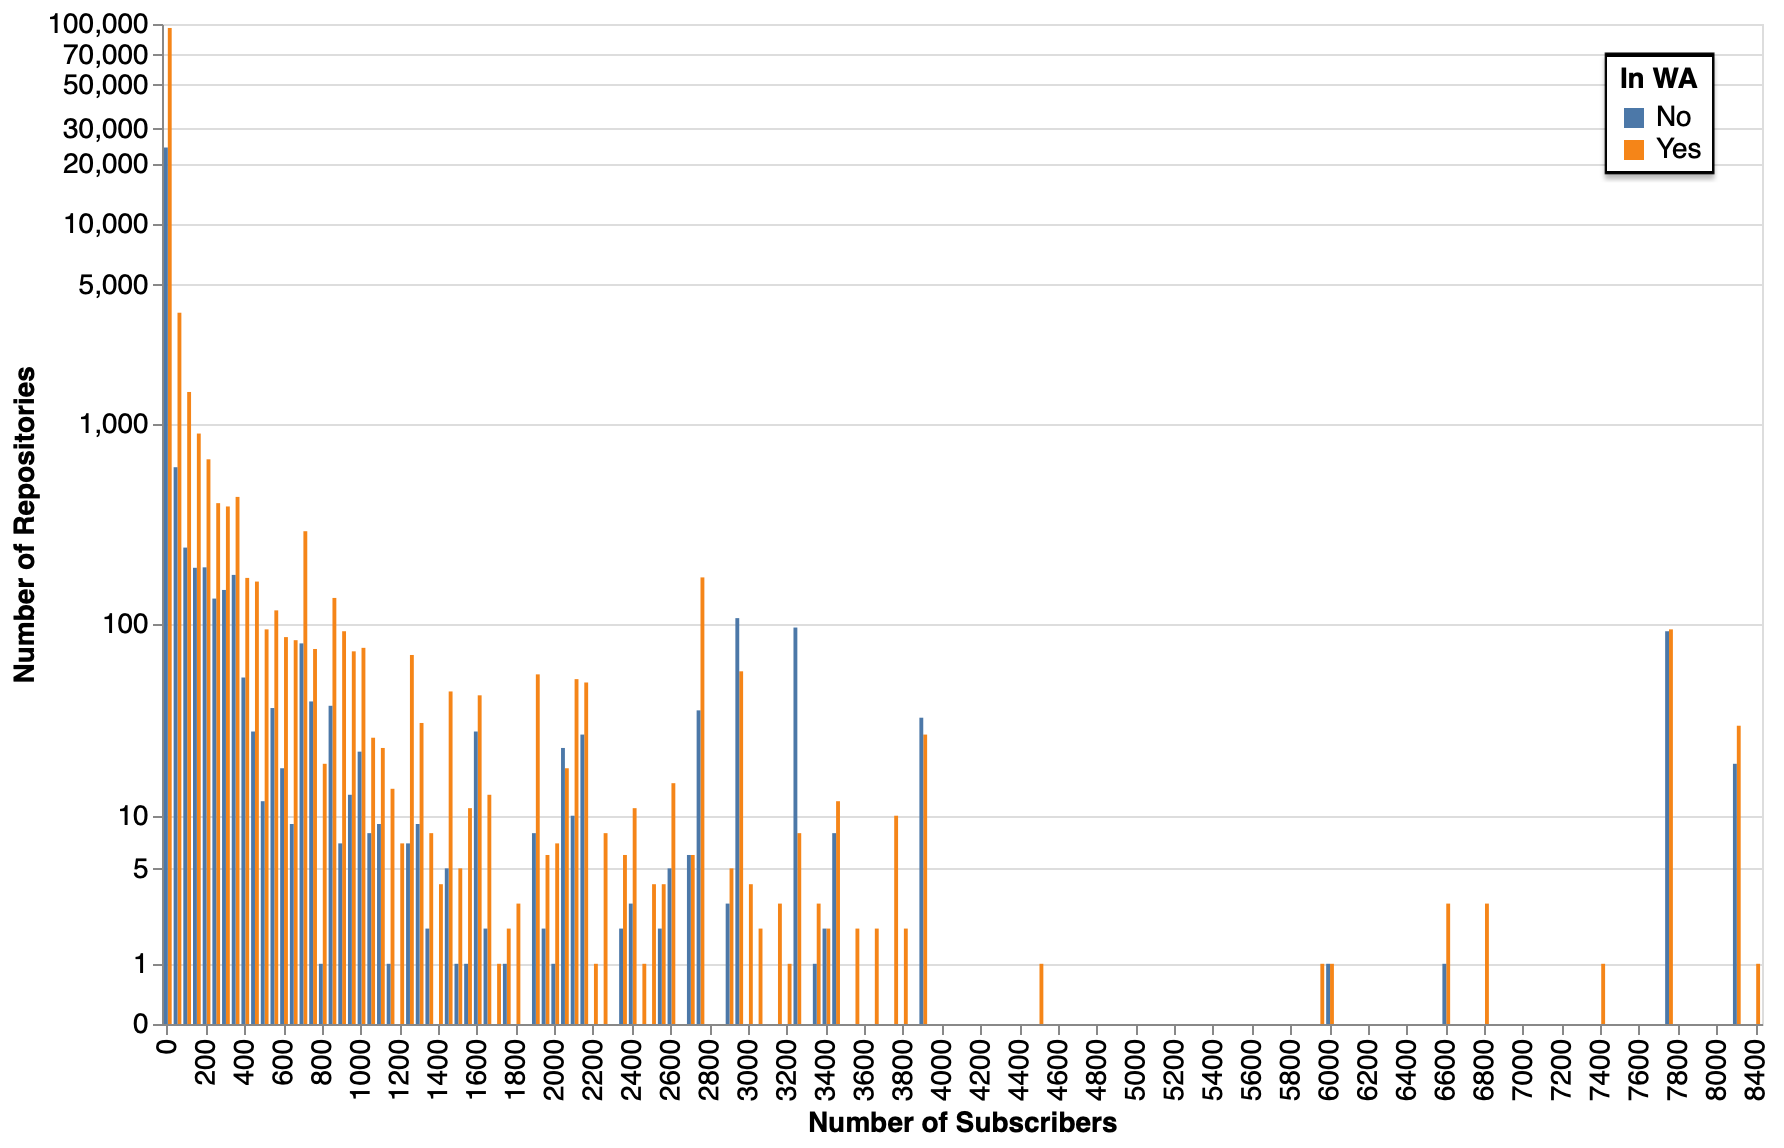
\includegraphics[width=\textwidth]{wa_subs.png}
    \caption{The distribution of subscribers for repositories archived and not archived in Web archives}
    \label{fig:wa_subs}
\end{figure}

\begin{figure}
    \centering
    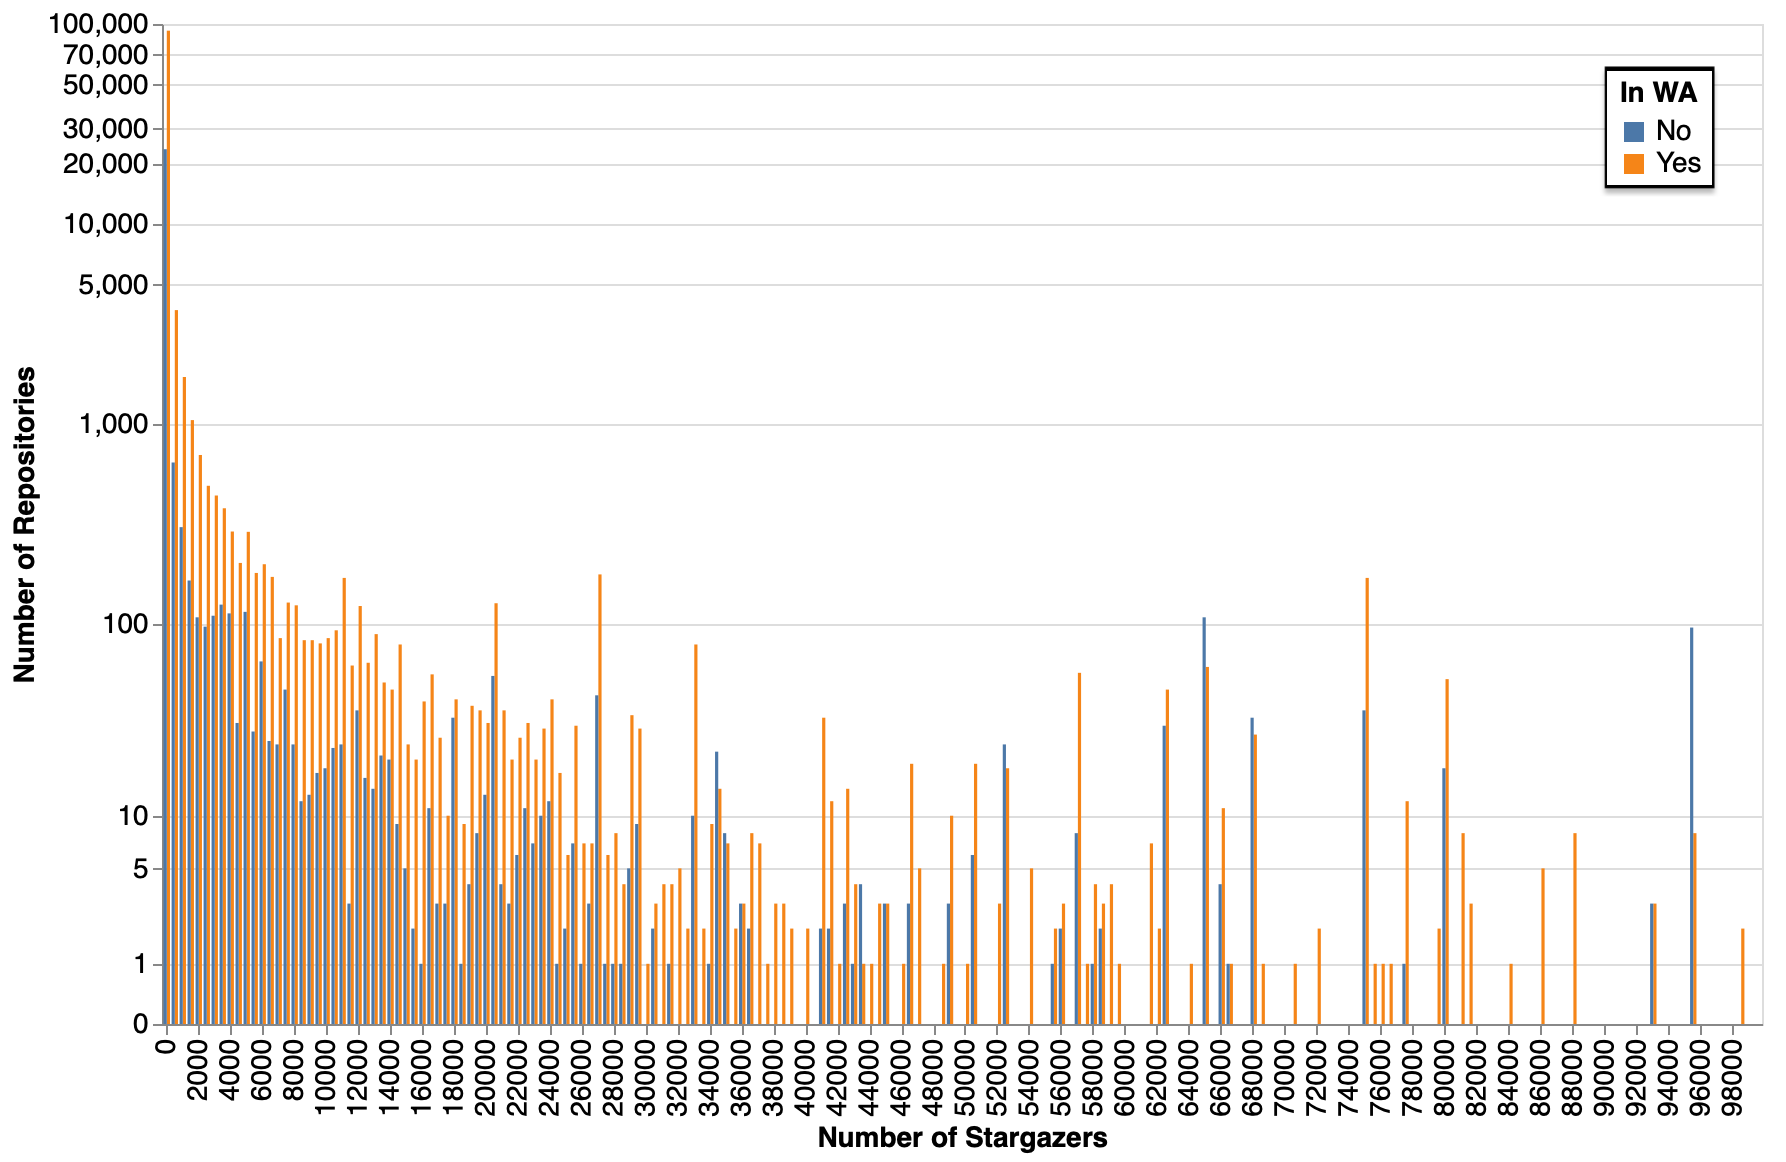
\includegraphics[width=\textwidth]{wa_stars.png}
    \caption{The distribution of stargazers for repositories archived and not archived in Web archives}
    \label{fig:wa_stars}
\end{figure}

\section{Discussion}

\section{Summary}
